\section{Montaggio Amplificatore}
Si è montanto il circuito come in \fig{setup_ampli}. Si è variata la resistenza del potenziometro in modo da ottenere una corrente di quiescienza pari a metà di $I_{dss}$ .Utilizzando $R_2 =\SI{227(3)}{\ohm} $ si è ottenuto il punto di lavoro: \\
$I_{d}^{Q}=\SI{6.8(1)}{\mA}$ \\
$V_{ds}=\SI{9.9(2)}{\V}$\\
$V_{gs}=\SI{-1.25(1)}{\V}$\\
Poichè $V_{ds} > V_{gs}-V_p $ il transistor è in regime di saturazione. Utilizzando i valori misurati prima per $I_{DSS}$ e $V_P$, si ricava la corrente di drain prevista $I_D = (I_{DSS}/V_P^2)(V_{GS} - V_P)^2 = \SI{7.09 (14)}{\mA} $, essenzialmente in accordo con quanto misurato.
Si è stimata poi la transconduttanza $g_m= \frac{2I_{dss}}{\left | V_p \right |}\sqrt{\frac{I_d}{I_{dss}}} $ che risulta :\\
$g_m = \SI{4.40 \pm 0.08}{\milli\siemens}$\\
Citiamo indicativamente il fatto che tale valore è compatibile con quello riportato sul datasheet per $V_{GS}=0$, che varia in un intervallo di \SIrange{2}{6.5}{\milli\siemens}. 
\begin{figure}[h]
	\centering
	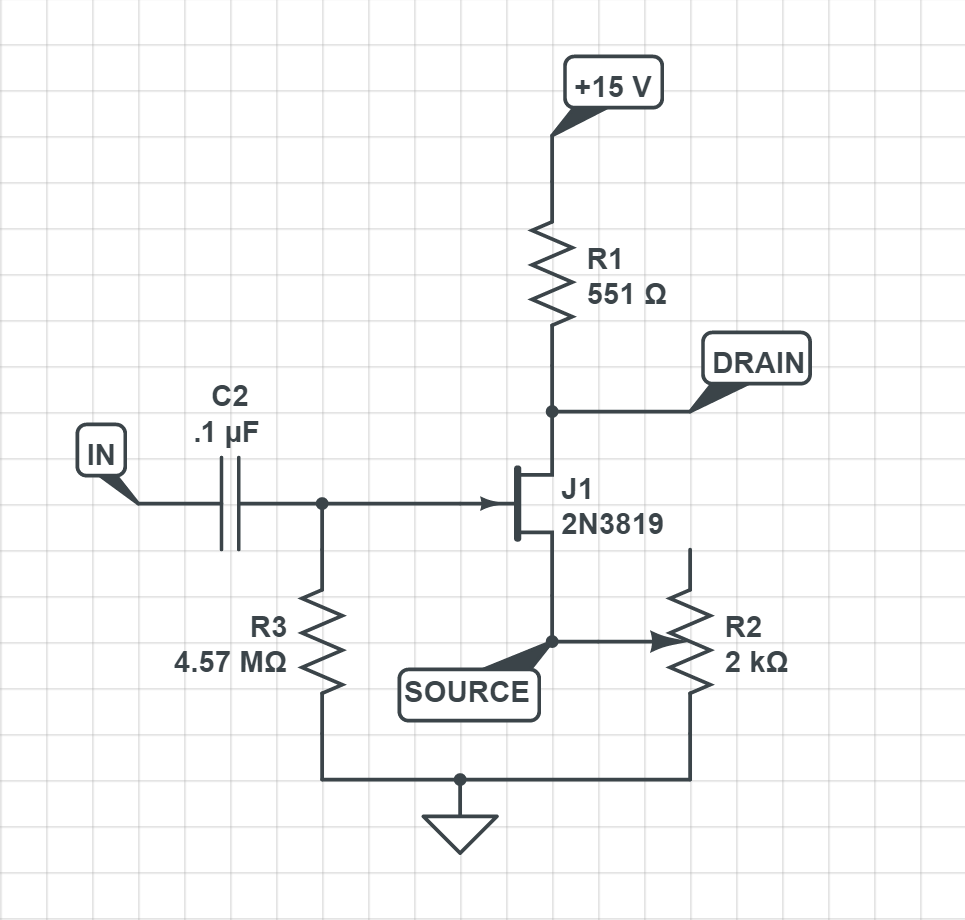
\includegraphics[scale=0.33]{amplisetup.png}
	\caption{Montaggio del circuito ampli.}
	\label{f:setup_ampli}
\end{figure}
